In this chapter, we will explain the fundamentals and technologies that have been used for the experimentation. We will focus on three main aspects:
\begin{enumerate}
\item The used dataset.
\item The used libraries for the development of the code.
\item Analysis of the code itself.
\item The used metrics to evaluate the obtained results.
\end{enumerate}

The idea of the experimentation part is to test and compare the frameworks that we have presented in Chapters \ref{Chapter:SimCLR} and \ref{Chapter:BYOL}. Their architectures have already been explained, and the original code for both backbones has not been done by me. 

This work will focus on testing how changing the training hyperparameters of the model affects the final results, since the original papers \cite{chen_simple_2020,grill2020bootstrap} already mention that using their structure, the results are affected by those hyperparameters, such as batch size, network depth or network width.

The implementations that have been used can be found in:
\begin{itemize}
\item SimCLR implementation: Official implementation from Google in \url{https://github.com/google-research/simclr/tree/master/tf2}

\item BYOL implementation: not official, found in \url{https://github.com/garder14/byol-tensorflow2}. 
\end{itemize}

The non-oficial implementation of BYOL has been chosen because it uses \emph{Tensorflow}, which makes the implementations easier to understand. Also, the idea is to make use of \emph{Tensorboard}, a Tensorflow utility that helps with visualization and graph generation of the training and final results.


\section{The dataset: CIFAR10}

The computational resources that we have for the experiment are limited. Due to this, we must fix a dataset that, having enough and representative examples, allows us to achieve feasible training time and successful results.

One of the ever most used dataset, which was also used in both SimCLR and BYOL papers, is CIFAR10 \citep{krizhevsky_learning_nodate}. This dataset will be used to test the overall performance of our representation learning methods.

CIFAR10 contains $60.000$ images divided in $10$ classes, where each class contains $10.000$ images. The size of the images is $32\times 32\times 3$, so the size of the images is not very large. This helps us to have faster trainings.

\begin{figure}[H]
    \centering 
    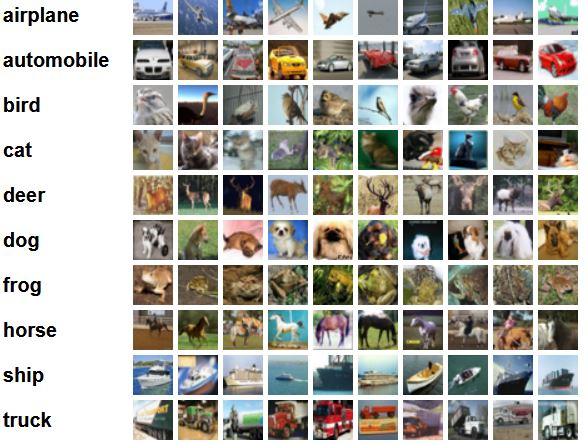
\includegraphics[scale=0.8]{CIFAR10}
    \caption{Ten examples of each class in the CIFAR10 dataset. }
\end{figure}
This dataset has $50.000$ samples for training and $10.000$ for test. The test batch contains the same number of examples of each of the $10.000$ classes in the dataset, that is, it contains $1.000$ examples of each class. 

It is important to remark that the classes are \emph{completely mutually exclusive}. That means that there is no overlap between the classes even if they have similar images, such as \emph{Cars} and \emph{Truck}, which are two of the classes of the dataset.

\section{Tensorflow}



Tensorflow\footnotemark is an open source library for developing machine learning frameworks.  

\begin{wrapfigure}{r}{5cm}
    \caption{Tensorflow logo.}
    
\includegraphics[scale=0.2]{tf-logo}
\end{wrapfigure}

%------------- Footnotemark
\footnotetext{Tensorflow documentation can be found at \url{https://www.tensorflow.org/}.}
%----------------------



It can be used for many tasks, but it focuses on training and inference of deep neural networks. It is used for both research and production at \emph{Google}, since it was also developed by the \emph{Google Brain} team for internal use. However, it was later released as open source.

The creation of new models is very simple, offering multiple abstraction levels. This is why it is suitable for our experimentations. Also, the code is very easily understandable.

There are other libraries that are widely used in machine learning algorithm development, such as \emph{Pytorch} or \emph{Jax}. However, Tensorflow has been chosen because of its simplicity and how common it is. 

\subsection{Tensorboard}

Tensorboard is a Tensorflow's visualization kit. It provides the visualization and tooling needed for machine learning experimentation. Among its more important utilities, we can find:
\begin{itemize}
\item Tracking and visualizing metrics (such as loss, accuracy, entropy) not only during the training but also when the training time has ended.

\item Visualizing the model graph: ops and layers.

\item Visualizing histograms of weights, biases and how tensors change during the training.

\item Projecting high-dimensional data to a lower dimensional space.

\item Displaying images,text and audio data.
\end{itemize}

Also, it is very easy to integrate with tensorflow.  Actually, in most of the cases it is as simple as adding the following \emph{callback} when we fit the model:

\begin{lstlisting}[language=python, caption=Integrating Tensorboard with Tensorflow.]

    tensorboard_callback = tf.keras.callbacks.TensorBoard
                        (log_dir=log_dir, histogram_freq=1)
    model.fit(x=x_train, 
              y=y_train, 
              epochs=5, 
              validation_data=(x_test, y_test), 
              callbacks=[tensorboard_callback])  

\end{lstlisting}




